\section{Beleuchtung}
In der Videografie wird die Belichtungszeit in der Bildrate vorgegeben, wohingegen sie in der Fotografie zwischen mehreren Stunden und wenigen Sekunden liegen kann.
Die richtige Belichtungszeit kann man sich mit folgender Formel berechnen: \textit{Belichtungszeit = 1: Framerate x 2}. Nimmt man nun mit 25 Bildern pro Sekunde auf, ergibt sich eine Belichtungszeit von 1:50 = 1/50 s. Würde man die Belichtungszeit verkürzen, z.B. auf 1/125 s, dann würde das Bild zwar schärfer werden, aber dann würde die Gefahr bestehen, dass der sogenannte Moir\'{e} Effekt eintritt. Der Moir\'{e} Effekt ist ein Bildfehler, der bei bewegten Bildern ein Flimmern erzeugt. \begin{quote}"Moir\'{e} tritt überall da auf, wo feine Muster oder Raster in einem gegeneinander verschobenen Winkel übereinanderliegen und sich gegenseitig beeinflussen." (Jörg Jovy, 2017, S. 211)\end{quote}
\begin{figure}[H]
	\centering
	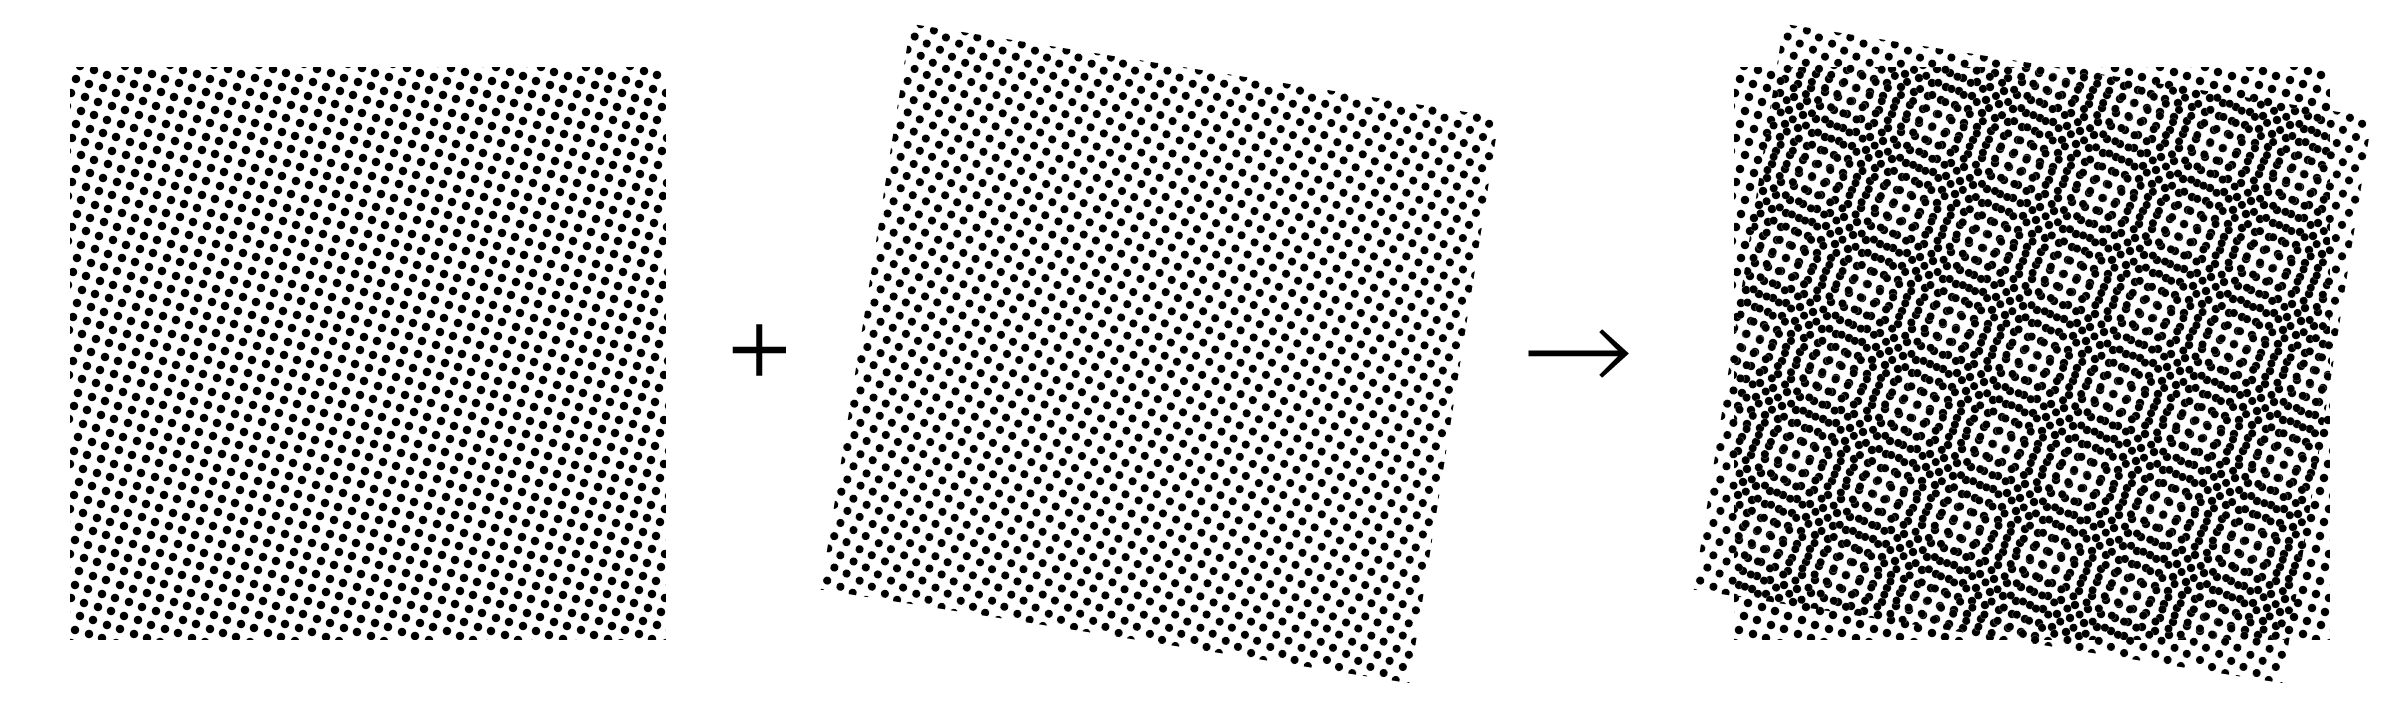
\includegraphics[width=0.8\textwidth]{abb2} 
	\caption[Moir\'{e}-Effekt]{Moir\'{e}-Effekt\footnotemark}
\end{figure}
\footnotetext{Quelle: https://de.wikipedia.org/wiki/Moir\%C3\%A9-Effekt\#/media/File:Moir\%C3\%A92.png}
Bei der Beleuchtung muss man drei Positionen von den Lichtquellen der Belichtung unterscheiden. Das Licht, das von vorne auf den Gegenstand kommt, nennt man Gegenlicht. Das Licht, das von der Seite kommt, wird als Streiflicht bezeichnet, und als drittes Licht wird das Auflicht verwendet, welches von hinten auf das Objekt scheint.\citep{beleuchtung}
\begin{figure}[H]
	\centering
	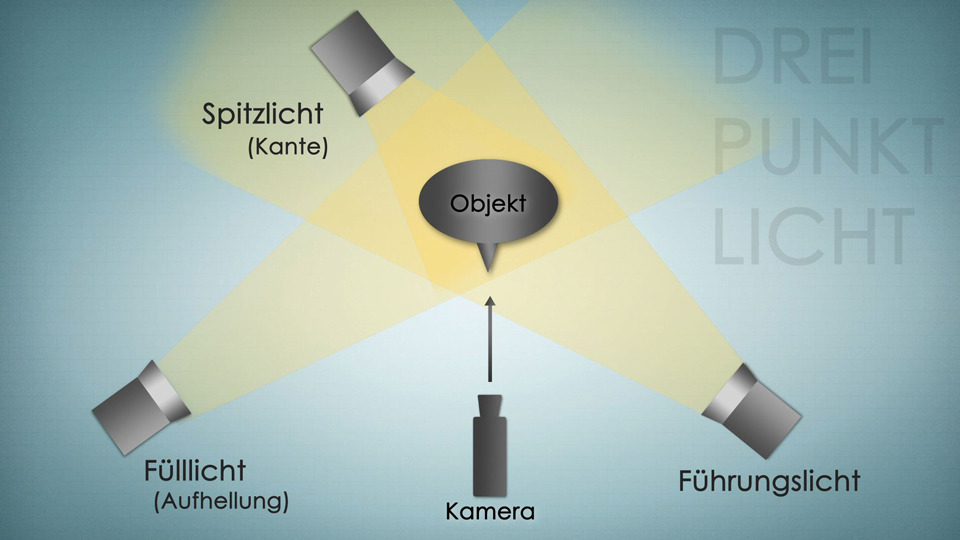
\includegraphics[width=0.7\textwidth]{abb3}
	\caption[Zusammenspiel der Lichter]{Zusammenspiel der Lichter\footnotemark}\label{fig:abb3}
\end{figure}
\footnotetext{Quelle: http://www.filmmachen.de/tipps-und-tricks/licht/3-punkt-beleuchtung}
Wie man auf der Abbildung \ref{fig:abb3} erkennen kann, ist es wichtig, wie die Lichter im Verhältnis zueinander stehen. Das Führungslicht, oder auch Hauptlicht genannt, dient dazu, die Szene generell aufzuhellen. Durch die Verwendung des Führungslichts entstehen Schatten, die wiederrum mit dem Fülllicht reduziert werden. Um den Gegenstand auch optisch vom Hintergrund abzuheben, kommt das sogenannte Spitzlicht zum Einsatz. \citep{lichter}
\paragraph{Softbox}
\leavevmode \\
Um den Schauplatz genügend auszuleuchten, wurden für alle vier Videos LED Scheinwerfer verwendet. Um keine harten Schatten zu erzeugen, wurden noch zusätzlich Softboxen verwendet.\newline
Eine Softbox ist im Grunde eine Hülle, bei der die Innenseite silber ist und welche dadurch das Licht wie ein Reflektor nach vorne reflektiert. Anschließend geht das Licht durch den "Front - Diffuser", was
ein lichtdurchlässiges Gewebe ist, der das Licht streut, und es so diffuser erscheinen lässt. Dadurch wird auch die Helligkeit reduziert und aufgrund der großen Fläche wird das Licht weicher, wodurch die Schatten diffuser werden.\citep{softbox}\newline
Bei dem Interview mit dem Abteilungsvorstand wurde jedoch keine 3-Punkt-Beleuchtung angewandt. Es wurde mit zwei Lichtquellen gearbeitet, um kein gekünsteltes Video zu erstellen. Die zwei Lichtquellen sollen nur dazu dienen, die Szene generell aufzuhellen und, um eventuelle Schatten auszugleichen. Es soll natürlich wirken und dem Betrachter nicht das Gefühl geben, dass es gestellt ist.  Dieses Set wurde ebenfalls bei dem Dreh des Quiz mit dem Absolventen und dem Schüler der zweiten Klasse angewandt, um auch hier ein natürliches Ergebnis zu erzeugen.